\documentclass[tikz,convert={outfile=kaczmarz.svg}]{standalone}
\usepackage{graphicx} % Required for inserting images
\usepackage{tikz}
\title{projection drawings}
\author{Nathaniel Pritchard}
\date{October 2025}
\definecolor{myred}{RGB}{203, 144, 77}
\definecolor{mygreen}{RGB}{195, 233, 145}
\definecolor{mynavy}{RGB}{81, 163, 163}
\definecolor{lager}{RGB}{223, 204, 116}
\definecolor{regal}{RGB}{117, 72, 94}
\begin{document}
       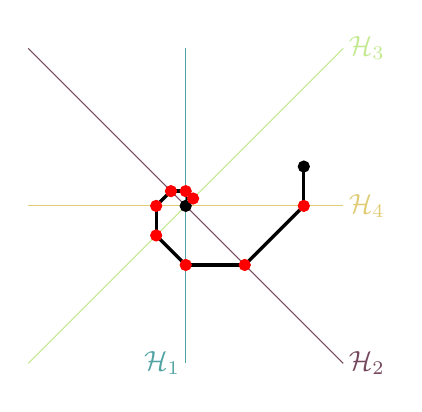
\begin{tikzpicture}
        \draw[color=mynavy] (0,0) -- (0,4);
        \node[color = mynavy] at (-.3,0) {$\mathcal{H}_1$};
        \draw[color=lager] (-2,2) -- (2,2);
        \node[color = lager] at (2.3,2) {$\mathcal{H}_4$};
        \draw[color=mygreen] (-2,0) -- (2,4);
        \node[color = mygreen] at (2.3,4) {$\mathcal{H}_3$};
        \draw[color=regal] (-2,4) -- (2,0);
        \node[color = regal] at (2.3,0) {$\mathcal{H}_2$};
        \filldraw[black] (0,2) circle (2pt);
        {\filldraw[black] (1.5,2.5) circle (2pt);}
        {\draw[very thick] (1.5,2.5) -- (1.5,2);}
        {\draw[very thick] (1.5,2) -- (.75,1.25);}
        {\filldraw[red] (1.5,2) circle (2pt);}
         {\draw[very thick] (.75,1.25) -- (0,1.25);}
         {\filldraw[red] (.75,1.25) circle (2pt);}
          {\draw[very thick] (0,1.25) -- (-.375, 1.625);}
          {\filldraw[red] (0,1.25) circle (2pt);}
          {\draw[very thick] (-.375, 1.625) -- (-.375,2);}
          {\filldraw[red] (-.375, 1.625) circle (2pt);}
          {\draw[very thick] (-.375,2) -- (-.1875, 2.1875);}
          {\filldraw[red] (-.375,2) circle (2pt);}
          {\draw[very thick] (-.1875, 2.1875) -- (0, 2.1875);}
          {\filldraw[red] (-.1875, 2.1875) circle (2pt);}
          {\draw[very thick] (0, 2.1875) -- (0.09374, 2.09374);}
          {\filldraw[red] (0, 2.1875) circle (2pt);}
          {\draw[very thick] (0.09374, 2.09374) -- (0, 2.09374);}
          {\filldraw[red](0.09374, 2.09374) circle (2pt);}
    \end{tikzpicture}
\end{document}
